\section{WattDepot}

Software for energy collection, storage, and analysis tends to come in two flavors that support two ends of the scalability spectrum.  At one end are utility-scale SCADA systems and protocols which are intended to manage macro-grid data \cite{SmartEnergy2.0, OSHAN, OpenPDC}.  At the other end are ``personal scale'' systems such as those provided by energy meter or solar panel manufacturers which are intended to manage information about single households \cite{TED, EMS100}.  We designed WattDepot to support a middle ground that we refer to as ``enterprise-level'' energy management, in which data concerning energy production and consumption of hundreds to thousands of households can be usefully managed~\cite{csdl2-10-05}. Figure \ref{fig:wattdepot} illustrates the architecture of the system, where WattDepot sensors send data from meters attached to energy devices to a server, which can then be queried by clients to provide visualizations and analyses.

\begin{figure}
\begin{center}
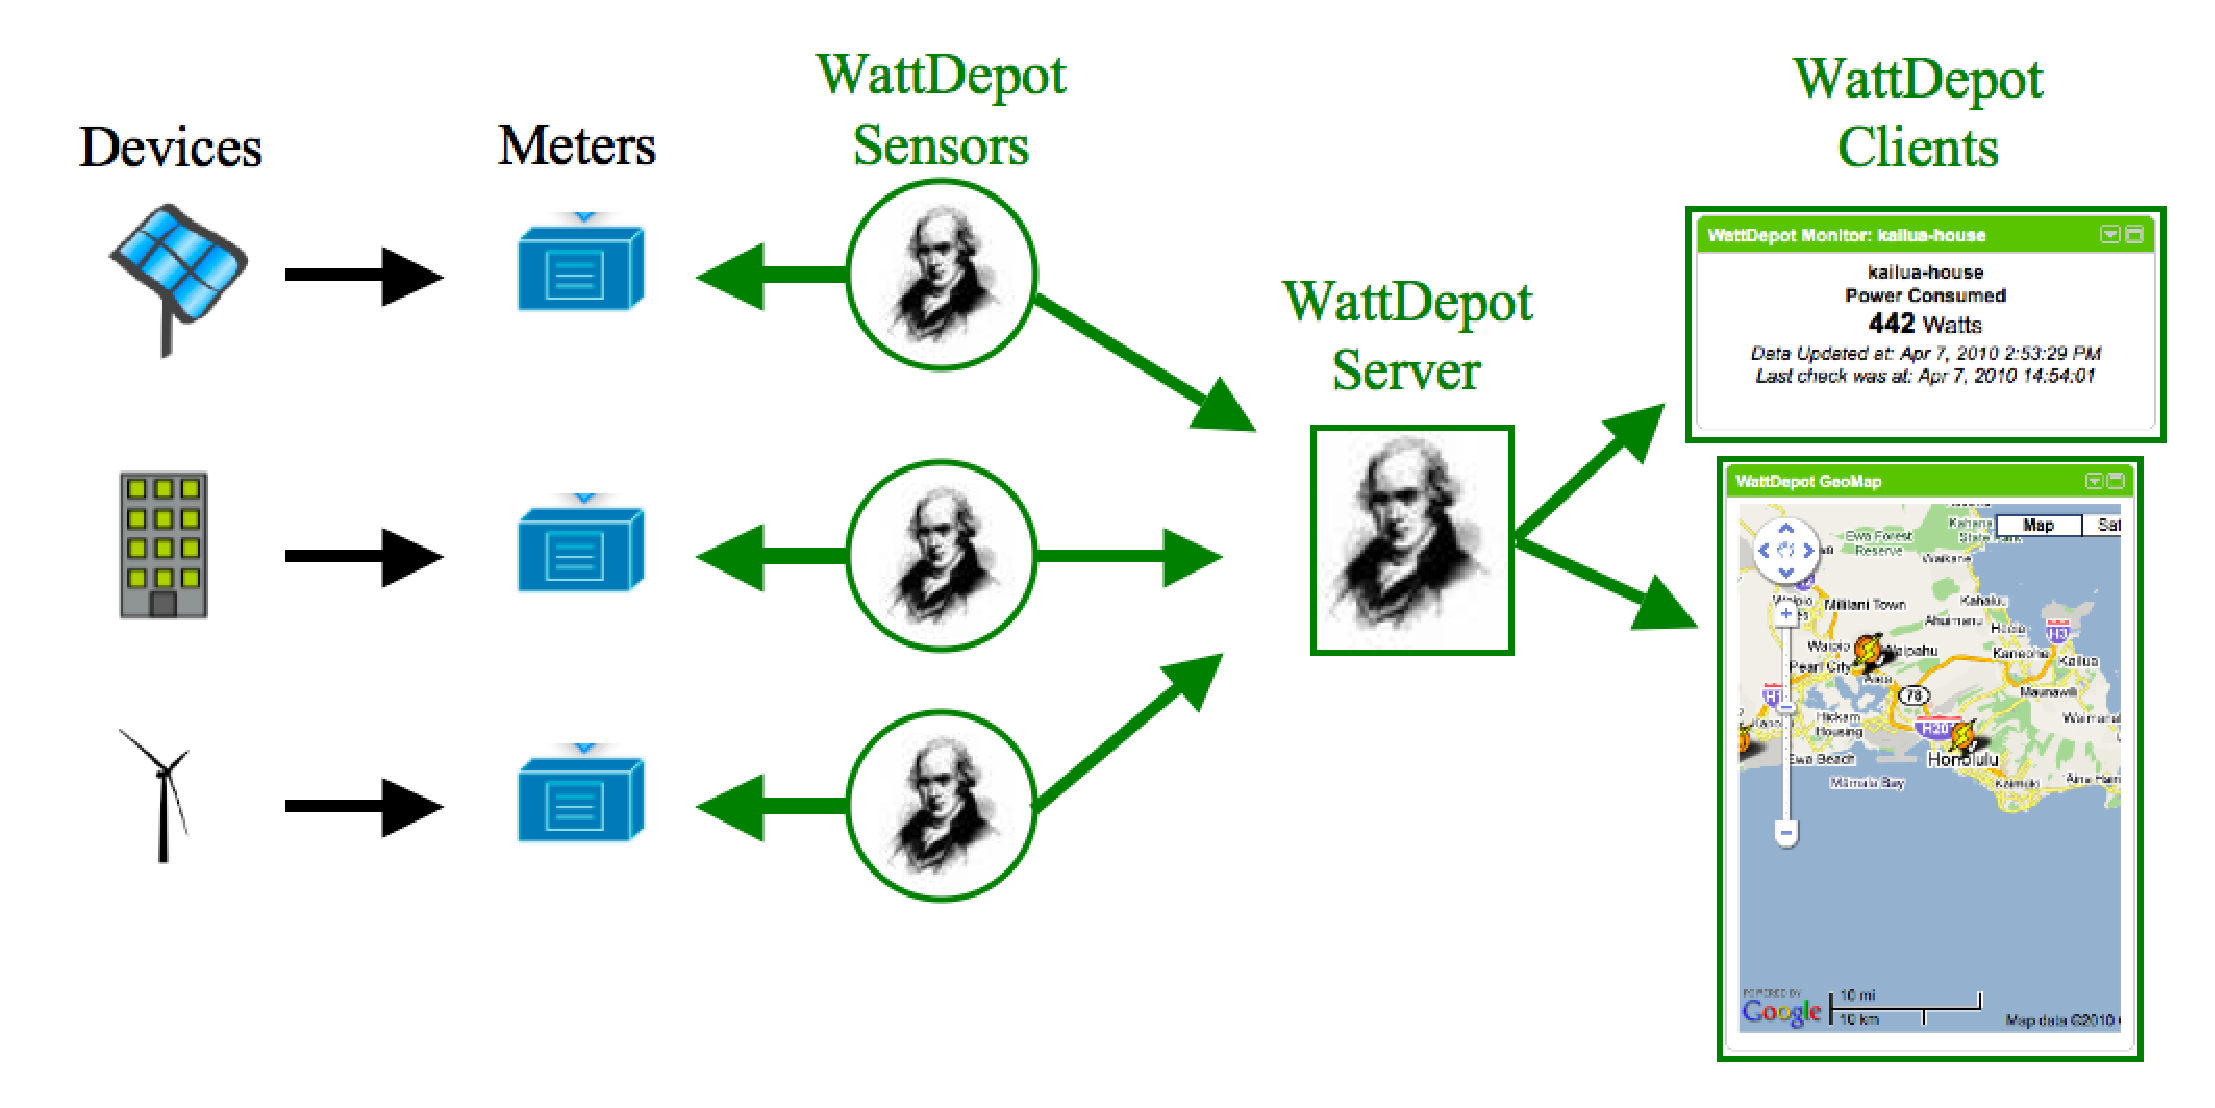
\epsfig{file=wattdepot-architecture, width=3in}
\end{center}
\caption{Architecture of WattDepot}
\label{fig:wattdepot}
\end{figure}

Our use of WattDepot has led to a novel set of capabilities to support this middle ground.

\subsection{Meter Agnostic}

Unlike personal-scale systems that are typically tied to a particular manufacturer's product, WattDepot is agnostic about the kinds of meters used to monitor energy production and consumption data, and whether the data is personal-scale or utility-scale. It provides a REST protocol for data transmission that can be used to implement clients for a wide variety of devices; the major constraint is that these devices need to have network access. WattDepot clients can be written in any language that supports the HTTP protocol. We provide a high-level client libraries for Java and JavaScript.

Due to the architectural decoupling of data collection from the rest of the system, WattDepot can be effectively used for simulation and what-if scenario development. This flexibility makes it appropriate as a kind of technological ``scaffolding'' for smart grid applications, where WattDepot can provide clients with simulated production and consumption data early in development, with the simulated data transitioning to live data as these sources go online later in development.

\subsection{Source Aggregation}

WattDepot can represent aggregations of power sou\-rces. For example, a building might have multiple meters monitoring energy consumption, one per floor. WattDepot can represent the power consumed by individual floors, as well as an aggregate source representing the building as a whole. Aggregations can be nested, so that floors can be aggregated into buildings, buildings into neighborhoods, and neighborhoods into cities. It is quite common for level of abstraction desired by client developers and end users (such as a floor of a building) to actually consist of multiple meters. By providing this aggregation of sources at the server level, client development becomes easier.

\subsection{Data Interpolation}

WattDepot automatically performs data interpolation when necessary. For example, a meter might provide a snapshot of energy usage once per hour for a given device. Clients can request the power consumed by this device at any time instant, and WattDepot will automatically provide interpolation when the requested time does not match a time for which actual sensor data is available. This is essential for the common case where meters do not have perfectly synchronized clocks and are not polled simultaneously, and when making use of the source aggregations discussed in the previous section.

\subsection{Flexible Data Storage}

WattDepot is architecturally decoupled from the underlying data storage technology. This supports experimentation with both traditional relational as well as NoSQL technologies, and facilitates scalability. Currently, WattDepot implements support for Derby, PostgreSQL, and BerkeleyDB storage systems. Administrators looking for simplicity may opt for the embedded Derby database, while those looking to integrate with existing database infrastructure might decide to use PostgreSQL for data storage.

WattDepot also implements support for ``ephemeral'' data. In some application scenarios, it is useful to send energy data to the WattDepot server quite frequently (i.e. every few seconds) so that clients can monitor current energy consumption with low latency. However, that rate of data sampling is not necessary for historical analyses, which may only require energy data sampling at the rate of every few minutes. WattDepot supports this situation through ephemeral data, which creates an in-memory window during which all recently received energy data is available for retrieval, but stored in the repository only at a much lower sampling rate.

\subsection{WattDepot in the Cloud}

In addition to installation on a local server, WattDepot has been designed to support cloud hosting, sometimes referred to as Platform-as-a-Service (PaaS). In particular, WattDepot can be deployed on the Heroku\footnote{http://www.heroku.com} cloud-based hosting service. The Heroku PaaS solution allows users to deploy the system and start collecting data without the requirement of server hardware, and Heroku offers flexible capacity depending on the expected workload.

\subsection{Beyond WattDepot}

While WattDepot provides the software infrastructure to collect, store, and analyze energy data, ensuring that the data is collected reliably and accurately reflects reality requires additional effort. As an example, we will examine the steps required to collect data on electricity use in a building. First, the administrator should work with manager of the building to understand the electrical infrastructure: how is power distributed in the building, and how does the distribution relate to the goals to be accomplished through measurement? If electricity is to be monitored at the per-floor level, do the distribution panels match that segmentation?

If the building does not have meters already installed, the administrator will need to select a meter vendor and acquire the meters. The meters will typically need to be installed by licensed electricians. The administrator will need to verify that the installation was performed correctly by checking whether the received data agrees with the expected amount of usage. To allow WattDepot to collect data, reliable network connectivity must be provided for the meters. The meters will also need to be configured to support remote data collection.

If the building already has meters installed, the administrator will need to confirm that the meters are configured correctly and that the data they produce  is sane. When working with existing meter infrastructure, the WattDepot administrator may not have administrative access to the meters, so any configuration changes required may need to be requested from the meter administrator.

Once data collection has been established, the WattDepot administrator will need to establish monitoring of the meters and WattDepot infrastructure so that hardware or software faults can be detected and corrected before they lead to excessive loss of data. By understanding these issues, administrators can ensure that systems built on top of WattDepot receive accurate energy data at appropriate levels of abstraction.
